\subsection{Modularisation}

To get a set of modules for the logical design, first consider the high-level structure of a \ac{cpu} seen in \autoref{fig:cpu_structure} in \autoref{sec:fundamentals_cpu_structure}. The \ac{alu} is an obvious choice for separating into a distinct functional module, as it literally implements an arithmetic function. Likewise, the control unit can be 
split into its own module. The \ac{isa} defines a set of 8 general purpose registers, all of which are homogenous and can therefore be abstracted away into a structure referred to as a register file. This way, the control logic and \ac{io} lines of each individual register can be shared and the entire file can be reasoned about at a higher level. Since there are many types of memory that can be used in an implementation, it makes sense to abstract the specific memory into a generic one, which can then provide a suitable interface to other modules. All memories, including the program counter, program memory, control signal memory and working memory are therefore split into separate modules. Finally, during development, the need for another module for controlling conditional branching became apparent. It also becomes its own module. At this point, an overview of each module, including its function and inputs and outputs is given.

\subsubsection{Arithmetic logic unit}

The \ac{alu} applies an arithmetic function to two binary numbers and outputs another binary number. It also outputs a set of status flags that inform the programmer about certain qualities of the result. This set of flags is described further in \autoref{sec:implementation_isa_memory_model}. Some \ac{alu} functions use the carry status bit from a previous operation as an additional input. Examples of this are the addition and subtraction functions, as well as the bit-shifting operators, in which the carry status bit determines the value of the bits to be inserted. The \ac{alu} must also know which of its functions to apply, therefore the \ac{alu}-opcode must be passed as an input, too. \autoref{tab:implementation_logical_alu_io} shows a list of all inputs and outputs to the \ac{alu} module.

\begin{table}[H]
    \centering
    \begin{tabular}{|l|l|l|} 
        \hline
        \textbf{\textbf{Signal}} & \textbf{Bits}           & \textbf{Description}                             \\ 
        \hline
        Opcode                   & 3                       & Selects the arithmetic function to be performed  \\ 
        \hline
        Operand A                & 8                       & The first operand of the arithmetic function     \\ 
        \hline
        Operand B                & 8                       & The second operand of the arithmetic function    \\ 
        \hline
        Carry In                 & 1                       & The carry-out status flag of the last operation  \\
        \hline
    \end{tabular}
    \label{tab:implementation_logical_alu_io}
    \captionof{table}{Input and output signals of the Arithmetic logic unit}
\end{table}

\subsubsection{Register}

Each register stores one word of data. It continuously outputs its current value and may be written to in a synchronous manner. Therefore, it must receive a clock input, as well as another input to be able to select if the register shall be written to upon the next clock cycle. This input is referred to as the ``Write enable'' line. To clear the value and reset the register, a ``Clear'' input is required. In order to read and write data, which may occur simultaneously, two 8 bit wide connections are required. \autoref{tab:implementation_logical_register_io} shows a list of all inputs and outputs to the register module.

\begin{table}[H]
    \centering
    \begin{tabular}{|l|l|l|} 
        \hline
        \textbf{\textbf{Signal}} & \textbf{Bits}           & \textbf{Description}                               \\ 
        \hline
        Data In                  & 8                       & Data to be written                                 \\ 
        \hline
        Data Out                 & 8                       & Readout of the currently stored data               \\ 
        \hline
        Clock                    & 1                       & Controls timing of data writing                    \\ 
        \hline
        Write Enable             & 1                       & Control if data is written or not                  \\ 
        \hline
        Clear                    & 1                       & Asynchronously writes the value 0 to the register  \\
        \hline
    \end{tabular}
    \label{tab:implementation_logical_register_io}
    \captionof{table}{Input and output signals of an individual register}
\end{table}

\subsubsection{Register file}

Since it is not feasible for an implementation to provide a set of control lines and \ac{io} lines for each individual register, a sharing mechanism is required. As there are 8 registers in the register file, $log_2(8) = 3$ bits are required to select a single one. From the instruction encoding described in \autoref{sec:implementation_instruction_encoding}, it is clear that an instruction can simultaneously read from two registers and write to another one. Therefore, each of these accesses requires its own selection input, totaling 9 bits. As only one register is written to at a time, all registers can share their write-enable, clock and data inputs. The register file module has only one of each and distributes it to all its register submodules. Similarly, all registers can share their ``clear'' signal, since no instruction defined in the \ac{isa} requires clearing of a single register. If needed, a programmer can load the constant value 0 from register \texttt{R0} into the desired register to clear it. In addition to general purpose registers, the flags register can be written to simultaneously. Therefore, two sets of write enable and data inputs are required. Also, since the content of the flags register may be needed for computation or branching decision making, it too is output continuously. Likewise, for memory access or branching instructions, the concatenated contents of registers \texttt{R6} and \texttt{R7} are read constantly. \autoref{tab:implementation_logical_register_file_io} shows a list of inputs and outputs of the register file module.

\begin{table}[H]
    \centering
    \begin{tabular}{|l|l|l|} 
        \hline
        \textbf{\textbf{Signal}} & \textbf{Bits} & \textbf{Description}                                \\ 
        \hline
        Read Select 0            & 3             & Selects the first register to read from             \\ 
        \hline
        Read Select 1            & 3             & Selects the second register to read from            \\ 
        \hline
        Write Select             & 3             & Selects the register to write to                    \\ 
        \hline
        Clear                    & 1             & Asynchronously writes the value 0 to all registers  \\ 
        \hline
        Clock                    & 1             & Controls timing of data writing                     \\ 
        \hline
        Write General Purpose    & 1             & Control if general purpose data is written or not   \\ 
        \hline
        Write Flag               & 1             & Control if flag data is written or not              \\ 
        \hline
        Data In General Purpose  & 8             & Data to be written to write-selected register       \\ 
        \hline
        Data In Flag             & 8             & Data to be written to flags register                \\
        \hline
        Data Read 0              & 8             & Data read from register selected by Read Select 0   \\
        \hline
        Data Read 1              & 8             & Data read from register selected by Read Select 1   \\
        \hline
        Data Read Flags          & 8             & Data read from the flags register R5                \\
        \hline
        Data Read Address        & 16            & Data read from the registers R6 and R7              \\
        \hline
    \end{tabular}
    \label{tab:implementation_logical_register_file_io}
    \captionof{table}{Input and output signals of the register file}
\end{table}

\subsubsection{Multiplexer} \label{sec:implementation_modularisation_multiplexer}

A multiplexer selects one of multiple inputs and outputs it unchanged. To select between $n$ input signals, $\lceil log_2(n)\rceil$ selector signals are required. For example, two select between 3 different input signals, a 2 bit wide selector signal is needed. Multiplexers can also have inputs and outputs that are $m$ bits wide. A multiplexer that switches between $n$ words of $m$ bits each is referred to as an ``m bit n:1 multiplexer''. All combinations of $n$ and $m$ can be built using only the basic 1 bit 2:1 multiplexer. Its output for the input signals $A$, $B$ and $S$ is determined by the boolean expression:

\begin{displaymath}
    (A \land \neg S) \lor (B \land S)
\end{displaymath}

\begin{figure}[H]
    \centering
    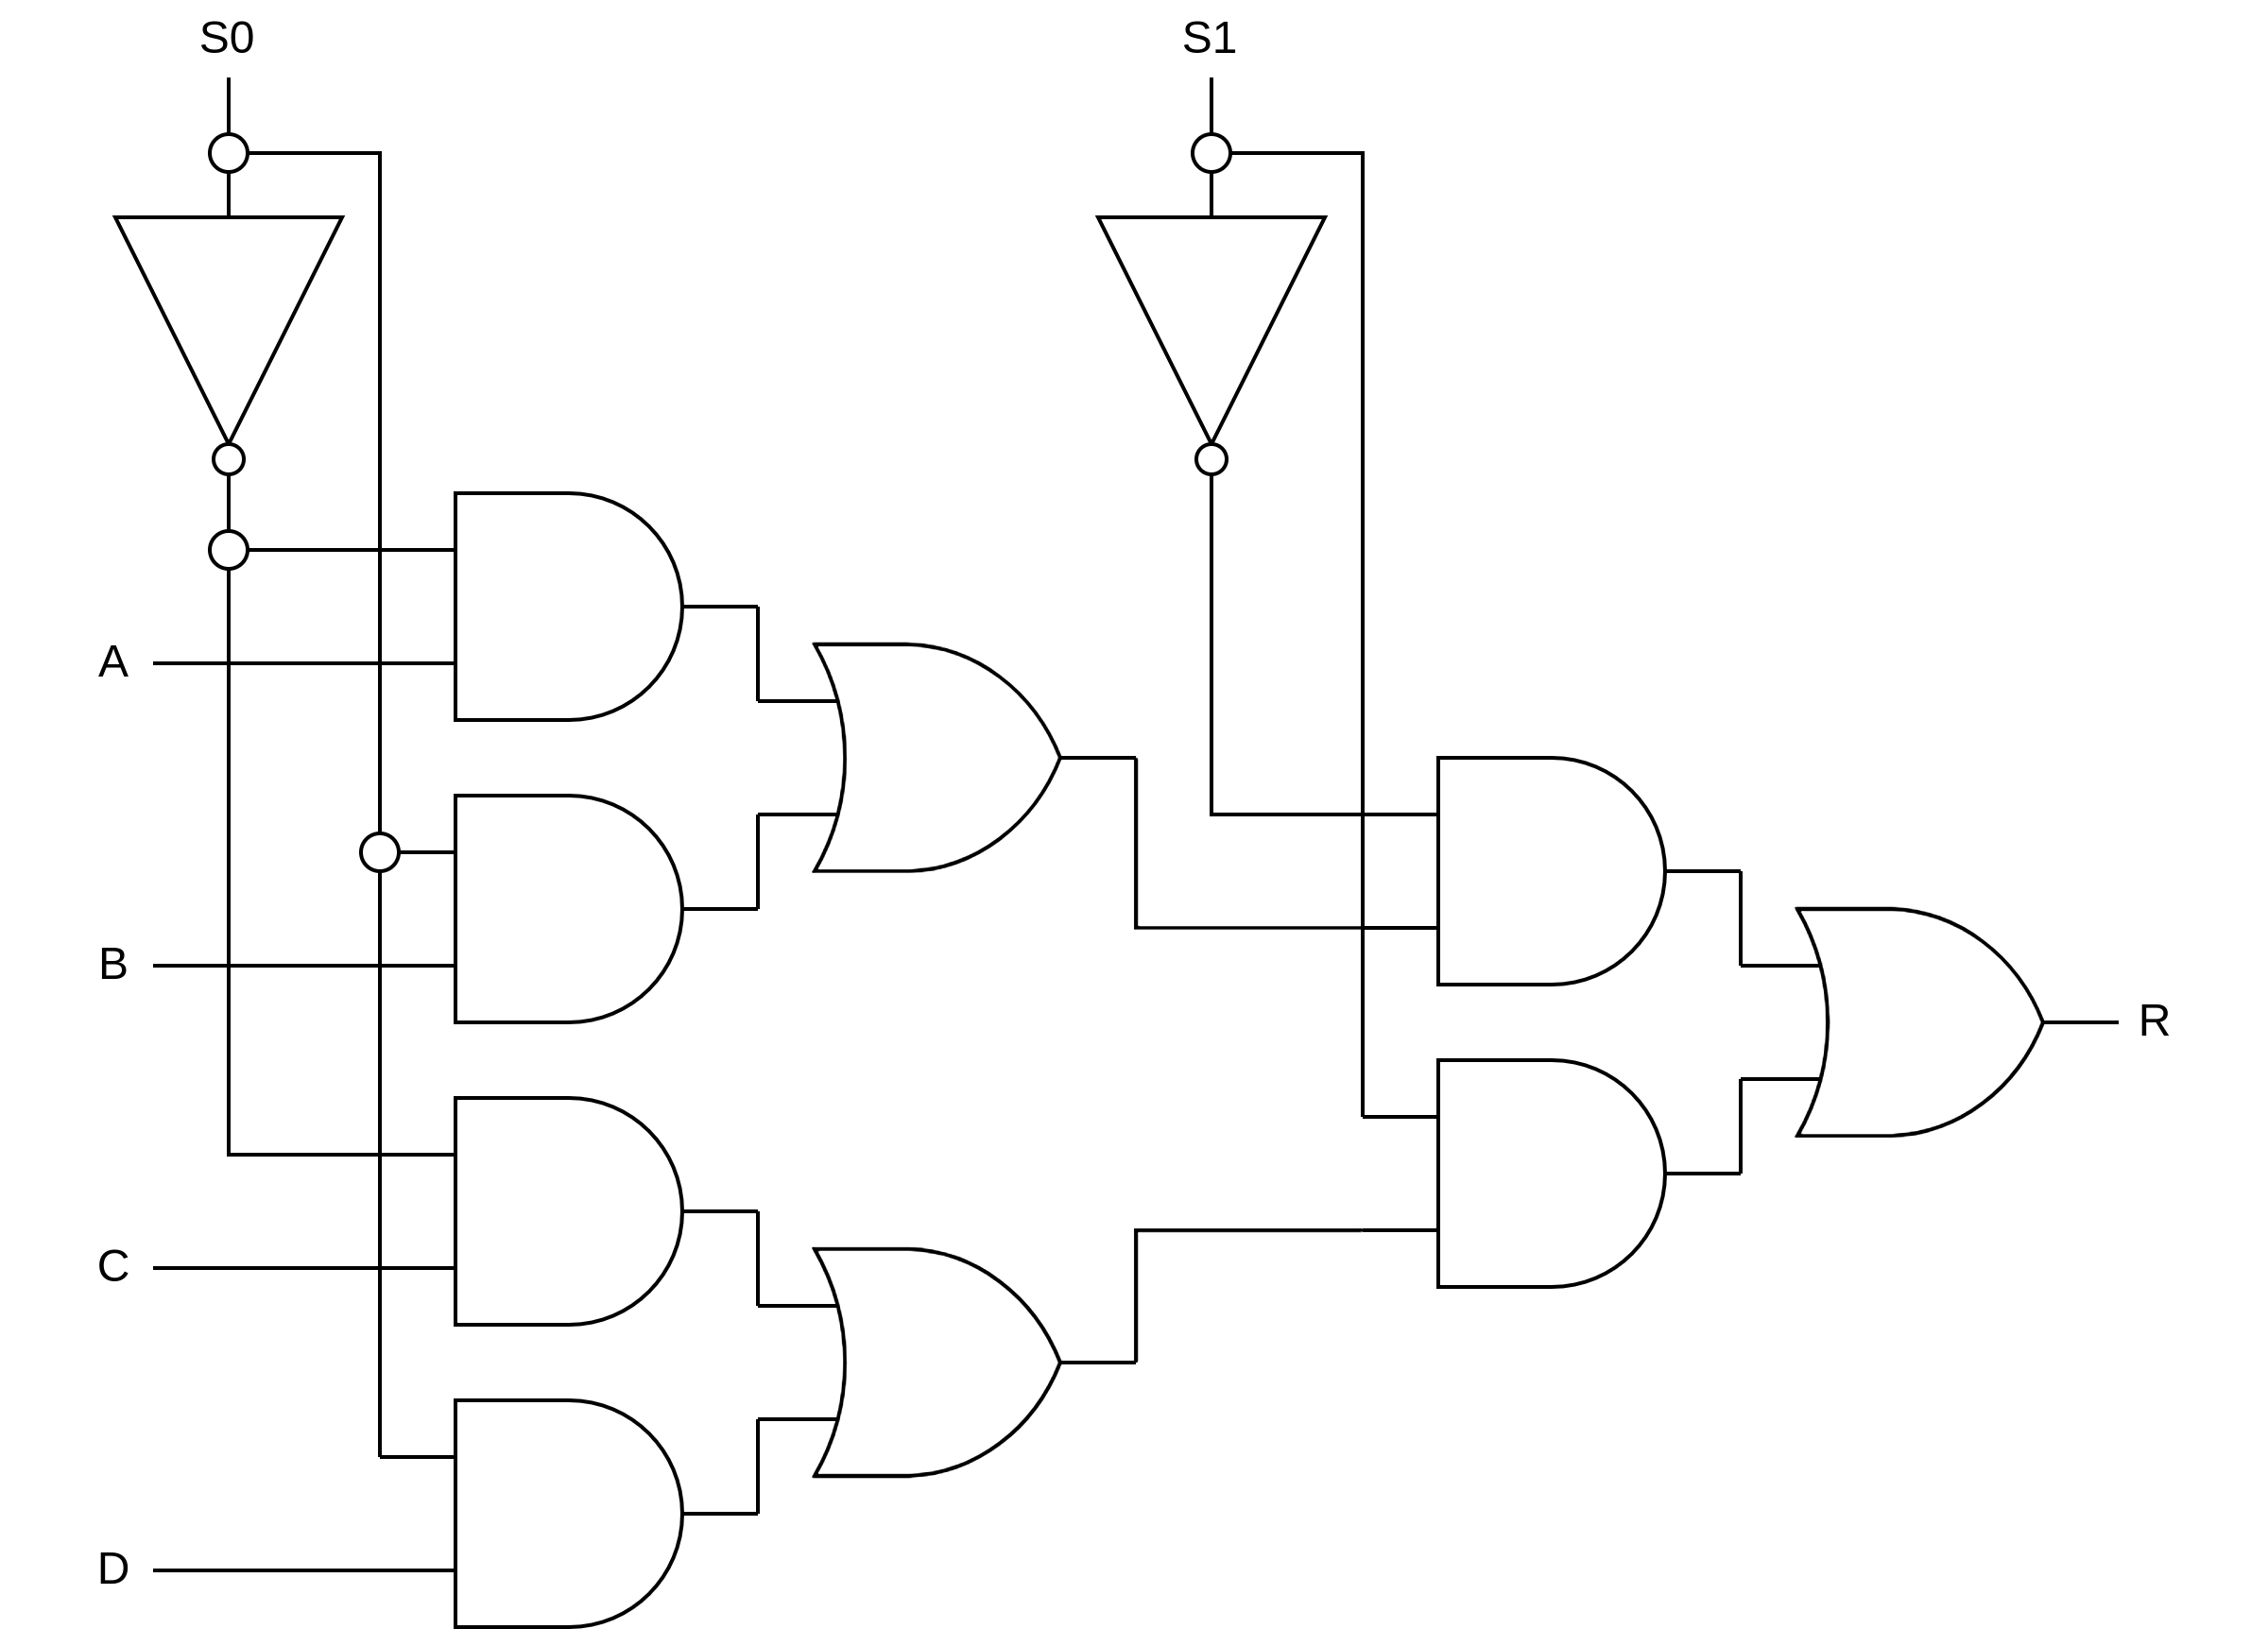
\includegraphics[width=0.7\textwidth]{images/drawio/multiplexer_tree.png}  % Replace with your image file
    \caption{1 bit 4:1 multiplexer from three 1 bit 2:1 multiplexers}
    \label{fig:implementation_modularisation_multiplexer_tree}
\end{figure}
To increase the number of inputs that can be selected from, a tree of 2:1 multiplexers is created. In this tree, the inputs of the leaves are the inputs of the resulting combined multiplexer. Each layer of the tree uses one bit of the selection input signal. By constructing a multiplexer this way, multiplexers with an arbitrary number of inputs can be constructed, provided the number of inputs is a power of two. This is a direct representation of a binary tree, since each individual 2:1 multiplexer serves as a tree node with two children. To increase the word size of a multiplexer, multiple n:1 multiplexers can be operated in parallel, again sharing their selection input signals. \autoref{fig:implementation_modularisation_multiplexer_tree} shows a 1 bit 4:1 multiplexer built from three individual 1 bit 2:1 multiplexers. For a filled, unskewed binary tree, the number of leaf nodes for a tree of height $h$ is given by $2^{h + 1} - 1$ \cite{tanenbaum2012sco}. Since each leaf multiplexer has 2 inputs, for an $m$ bit multiplexer of $n$ inputs, the following equation gives the number of 1 bit 2:1 multiplexers required in total:

\begin{displaymath}
    N_{multiplexers}(n, m) = m \times (2^{\lceil log_2(n) \rceil} - 1)
\end{displaymath}

As an example, an 8 bit 4:1 multiplexer requires 
\begin{displaymath}
    N_{multiplexers}(4, 8) = 8 \times (2^{\lceil log_2(4) \rceil} - 1) = 24
\end{displaymath}

1 bit 2:1 multiplexers.


\subsubsection{Control unit}

The AVA architecture is designed with the complexity of the control unit in mind. Therefore, the architecture can be implemented using only horizontal microcode. The opcode is directly used as an address to read-only memory referred to as control signal memory. This memory stores the control word for each operation. The control word is then output and can be used as a selector for multiplexers within the interconnection network between modules. The individual control signals of the control word can also be used to control the function of modules directly. Due to its simplicity, the control unit module has a single input, which is the opcode, and outputs $n$ control signals, where $n$ depends on the interconnection network. \autoref{tab:implementation_logical_control_unit_io} shows a list of inputs and outputs of the control unit.

\begin{table}[H]
    \centering
    \begin{tabular}{|l|l|l|} 
    \hline
    \textbf{\textbf{Signal}} & \textbf{Bits} & \textbf{Description}                                  \\ 
    \hline
    Opcode                   & 7             & Address for the control signal memory                 \\ 
    \hline
    Control Signals          & N             & Used for controlling data routing and module control  \\
    \hline
    \end{tabular}
    \label{tab:implementation_logical_control_unit_io}
    \captionof{table}{Input and output signals of the control unit}
\end{table}

\subsubsection{Memory}

The working memory must be addressable, therefore an address input is needed. Also, there must be two 8 bit connections for data \ac{io}. Lastly, the control unit must be able to instruct the memory on when data is read and written from the module, for which two dedicated control signals are used. In principle, all used memories are connected in this manner, however only the working memory must be writable. Both the program and control signal memory are read-only and do therefore not require control signals. The module is expected to interface with its environment in a synchronous, parallel manner, i.e there is no serialisation of data. This makes integration with other components simpler. However, an additional signal line must carry a clock signal to control timing. Many electrical memory components minimize the size of their package by using shared pins for data input and output. However, to simplify the logical design and clearly show the datapath within the device, distinct input and output connections are used.

\begin{table}[H]
    \centering
    \begin{tabular}{|l|l|l|} 
        \hline
        \textbf{\textbf{Signal}} & \textbf{Bits} & \textbf{Description}                    \\ 
        \hline
        Address                  & 16            & Address for the memory                  \\ 
        \hline
        Read Enable              & 1             & Controls when the memory outputs data   \\ 
        \hline
        Write Enable             & 1             & Controls when the memory is written to  \\ 
        \hline
        Clock                    & 1             & Controls read/write timing              \\ 
        \hline
        Data In                  & 8             & Data used for writing to memory         \\ 
        \hline
        Data Out                 & 8             & Data read from memory                   \\
        \hline
    \end{tabular}
    \label{tab:implementation_logical_memory_io}
    \captionof{table}{Input and output signals of a memory unit. Only working memory requires read-enable, write-enable and clock lines.}
\end{table}

\subsubsection{Branch control} \label{sec:branch_control_unit}

The branch control module is introduced to contain several logic gate components which would otherwise remain on the ``top level'' of the logic design. The purpose of this module is to determine if the program counter is to be incremented or loaded from a different source, effectively performing a branching operation. Since the contents of the control signal memory are constant and the branching decision requires dynamic information at runtime, combinatorial logic is needed to combine the dynamic and constant signals. The AVA \ac{isa} defines only the ``zero'' bit of the flags register to be used for branching decision making, as is explained in \autoref{sec:implementation_opcodes}. Therefore, the zero bit of the \ac{alu} flag output is combined with two control signals. The first one controls whether a conditional branch is executed. The second one selects whether to branch if the zero flag bit is set or unset. The output of the combinatorial circuit is then used as an internal control signal to control the source multiplexer for the program counter. \autoref{fig:implementation_modularisation_branch_control_logic} shows the simple internal logic of the unit. \autoref{tab:implementation_branch_control_io} shows a list of inputs and outputs of the branch control unit.

\begin{figure}[H]
    \centering
    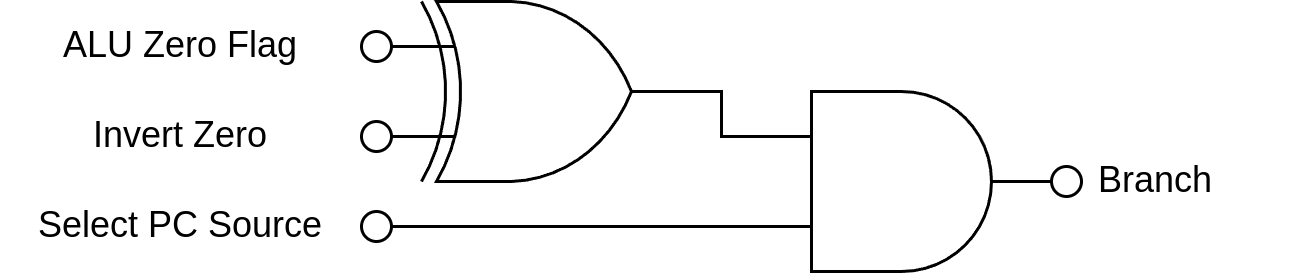
\includegraphics[width=0.7\textwidth]{images/drawio/branch_control.png}  % Replace with your image file
    \caption{Branch control unit logic}
    \label{fig:implementation_modularisation_branch_control_logic}
\end{figure}

\begin{table}[H]
    \centering
    \begin{tabular}{|l|l|l|} 
        \hline
        \textbf{\textbf{Signal}}      & \textbf{Bits} & \textbf{Description}                           \\ 
        \hline
        Zero Flag                     & 1             & Set when the ALU result contains only 0        \\ 
        \hline
        Invert Zero Condition         & 1             & Controls when the memory outputs data          \\ 
        \hline
        Select Program Counter Source & 1             & Selects whether a branch can occur             \\ 
        \hline
        Branch Control Signal         & 1             & Selects source for next program counter value  \\
        \hline
    \end{tabular}
    \label{tab:implementation_branch_control_io}
    \captionof{table}{Input and output signals of the branch control unit}
\end{table}
